\newSec[MusterObserver]{Beobachter}{3}

\newSec{Klassifikation}{4}
Objektbasiertes Verhaltensmuster\footnote{Anhand der Vorlesungsfolien \glq Entwurfsmuster Beobachter\grq}

\clearpage
\newSec{Struktur}{4}
\begin{figure}[ht!]
\vspace{0.25cm}
\begin{center}
\fbox{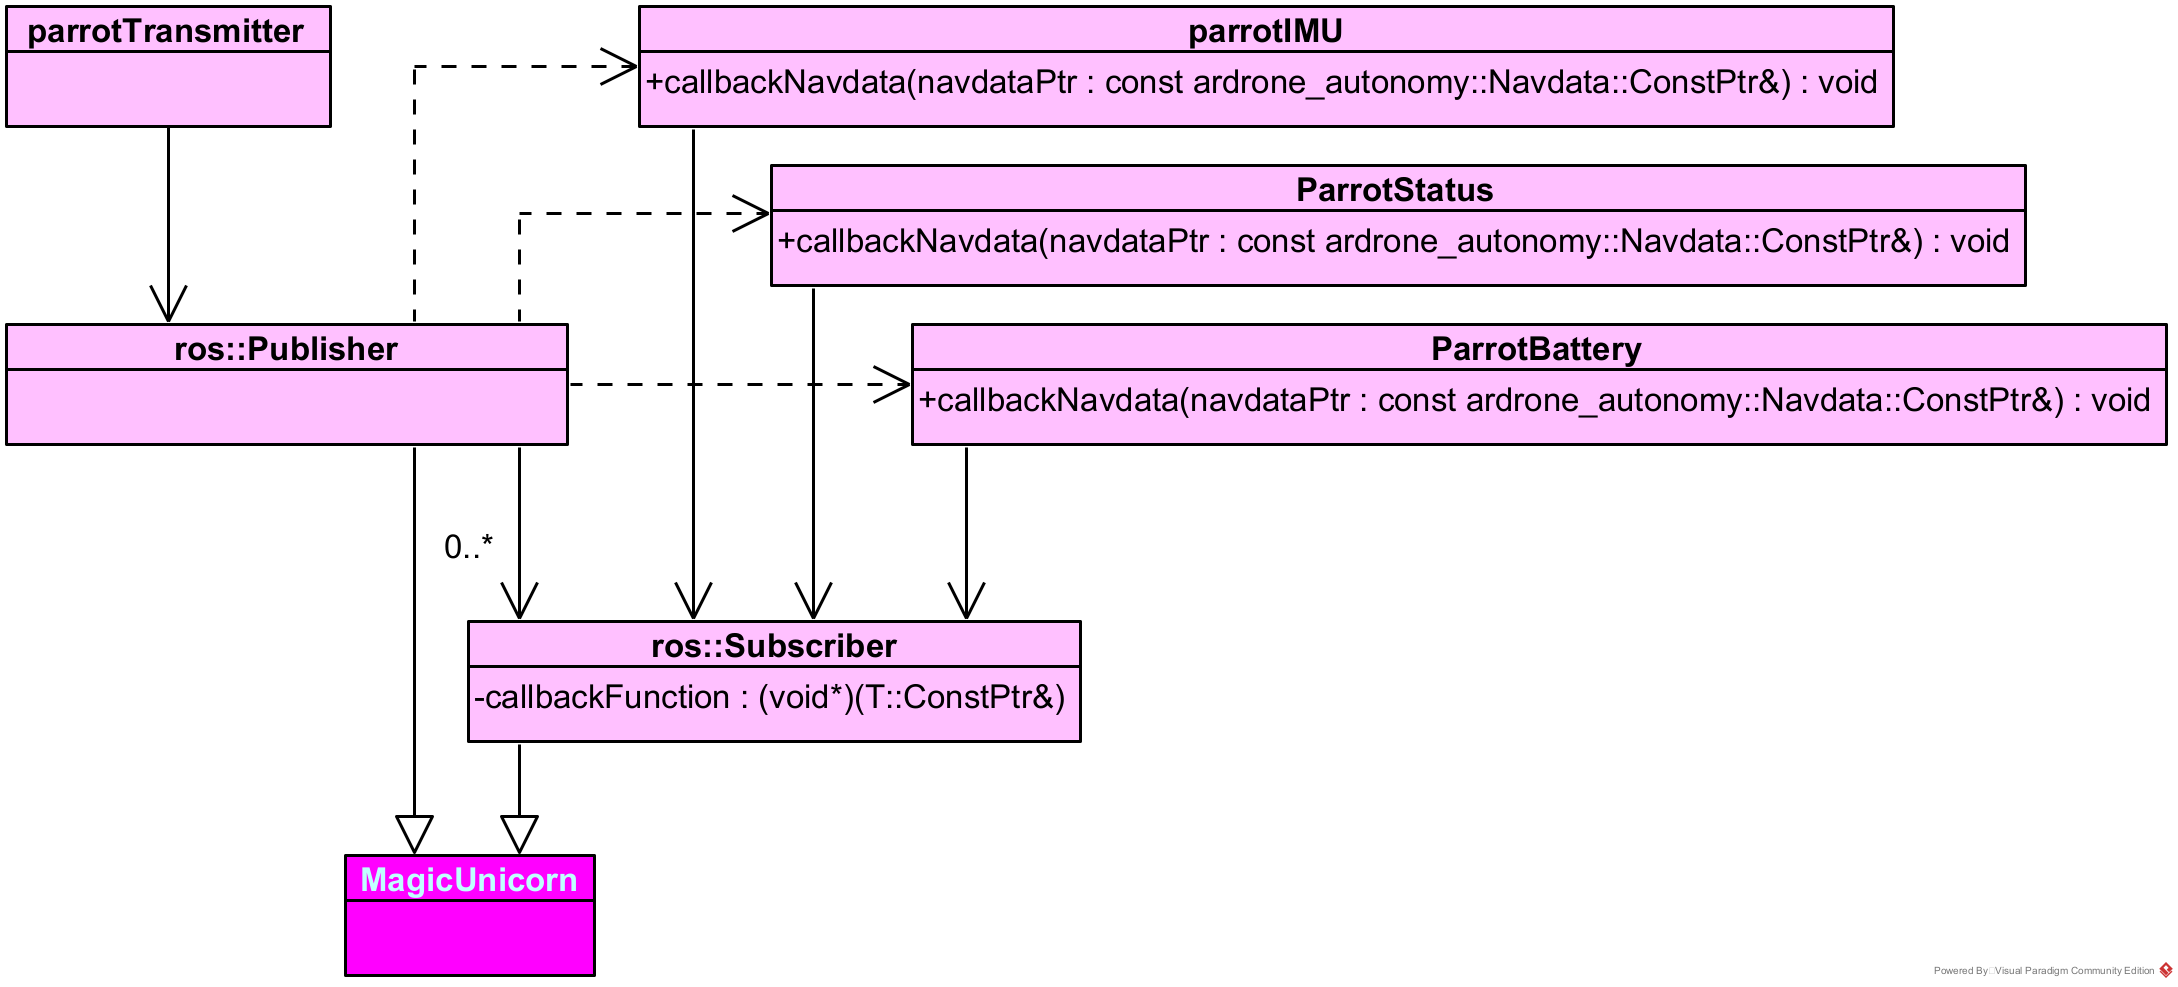
\includegraphics[width=15cm]{Pictures/Observer.png}}
\caption{Observer im Projekt}
\label{fig:Obs}
\end{center}

\vspace{0.25cm}
Im \ROS-Framework wird die Funktionalität mittels \textit{Function Pointer} an den Beobachter übertragen. Eine Vererbung findet nicht statt.\\
\note{Die in der Abbildung als \glqq MagicUnicorn\glqq bezeichnete Klasse ist in diesem Zusammenhang die Untiefen des \ROS-Frameworks, welches deutlich über das im verfügbaren Zeitraum aufbringbare Verständnis der Autor:innen hinausgeht.}
\end{figure}


\FloatBarrier
\newSec[Akteure]{Akteure\footnotemark[6]}{4}
\begin{table}[!ht]
\begin{tabular}{ll}
Akteur				& Klassenbezeichnung \\ \hline
Subjakt				& ros::Publisher\\
KonkretesSubjekt		& parrotTransmitter\\
Beobachter			& ros::Subscriber\\
KonkreterBeobachter 0	& parrotIMU\\
KonkreterBeobachter 1	& parrotStatus\\
KonkreterBeobachter 2	& parrotBattery
\end{tabular}
\end{table}


\FloatBarrier
\newSec{Motivation}{4}
Die \ROS-\Pub{} und \Sub{} kommunizieren über \Topic[s] miteinander. \comp{ROSObserer1} Die Drohne ist ausschließlich mittels \ROS\ erreichbar.

